\documentclass[12pt]{book}
\usepackage{pstricks}
\usepackage{amsmath,amssymb,graphicx,wasysym}
\usepackage{psfrag,pstricks,verbatim}
\usepackage[squaren]{SIunits}
\usepackage{multirow}

\topmargin=-0.5in
\oddsidemargin=0in
\evensidemargin=0in
\textwidth=6.5in
\textheight=9in
\parindent=0pt
\pagestyle{empty}
\begin{document}
Names\underline{\smash{ Brij Kapadia} \hspace{1in}} 
\begin{enumerate}
	\item The \verb|TableForm[]| below reveals some details about the \verb|ourFib[]| and \verb|fastFib[]| function we wrote in class, along with the built-in \verb|Fibonacci[]| function.
	\begin{center}
		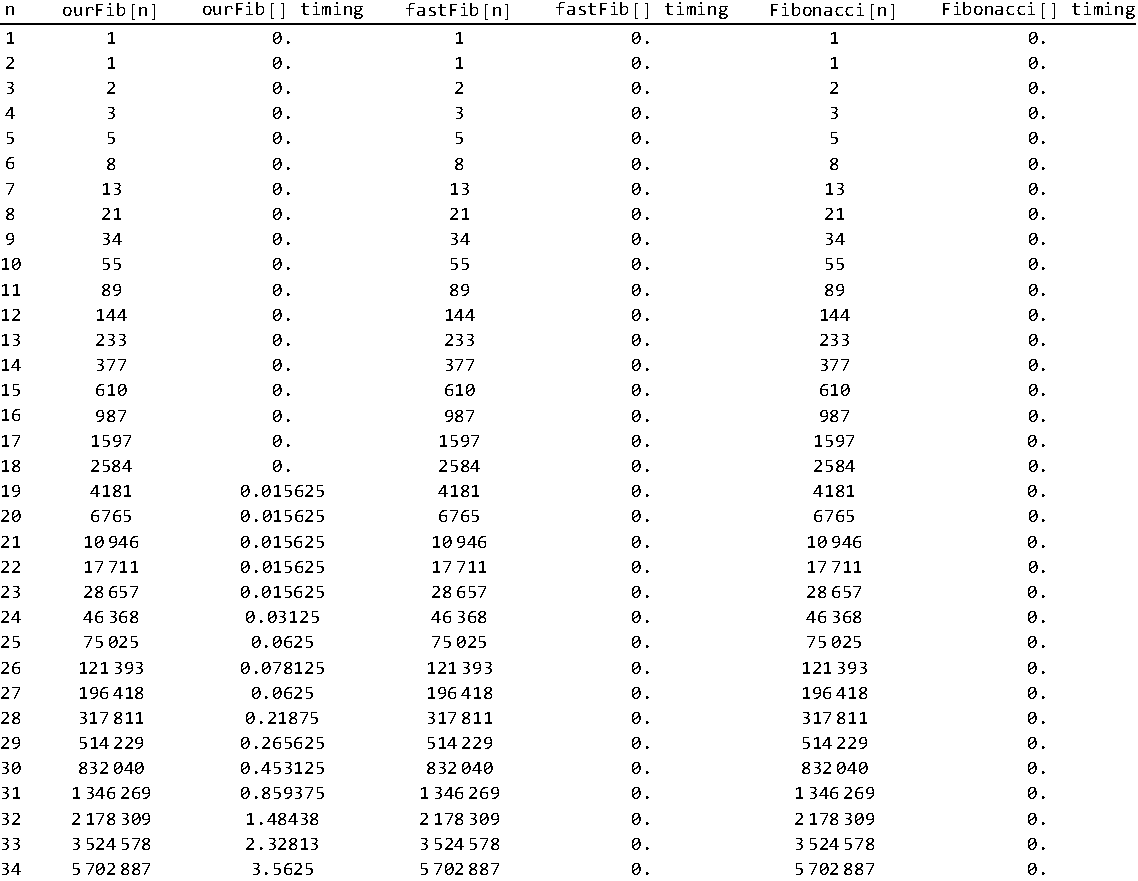
\includegraphics[width=6in]{table.pdf}
	\end{center}
	Generate this \verb|TableForm[]|, formatted exactly as shown.
	\newpage
	\item the \verb|array| below shows the function $f(x)=\dfrac{x}{1-x-x^2}$; hardly any of these values were actually typed in this \LaTeX \ document.
	\renewcommand{\arraystretch}{2}
	\begin{center}
		$$
		\begin{array}{||c|c|c||}
			\hline
			n & f^{(n)}(x) & f^{(n)}(x)/n! \\
			\hline
			0 & -\frac{x}{x^2+x-1} & 0 \\
			1 & \frac{x^2+1}{\left(x^2+x-1\right)^2} & 1 \\
			2 & -\frac{2 \left(x^3+3
				x+1\right)}{\left(x^2+x-1\right)^3} & 1 \\
			3 & \frac{6 \left(x^4+6 x^2+4
				x+2\right)}{\left(x^2+x-1\right)^4} & 2 \\
			4 & -\frac{24 \left(x^5+10 x^3+10 x^2+10
				x+3\right)}{\left(x^2+x-1\right)^5} & 3 \\
			5 & \frac{120 \left(x^6+15 x^4+20 x^3+30 x^2+18
				x+5\right)}{\left(x^2+x-1\right)^6} & 5 \\
			6 & -\frac{720 \left(x^7+21 x^5+35 x^4+70 x^3+63
				x^2+35 x+8\right)}{\left(x^2+x-1\right)^7} & 8
			\\
			7 & \frac{5040 \left(x^8+28 x^6+56 x^5+140 x^4+168
				x^3+140 x^2+64
				x+13\right)}{\left(x^2+x-1\right)^8} & 13 \\
			8 & -\frac{40320 \left(x^9+36 x^7+84 x^6+252
				x^5+378 x^4+420 x^3+288 x^2+117
				x+21\right)}{\left(x^2+x-1\right)^9} & 21 \\
			9 & \frac{362880 \left(x^{10}+45 x^8+120 x^7+420
				x^6+756 x^5+1050 x^4+960 x^3+585 x^2+210
				x+34\right)}{\left(x^2+x-1\right)^{10}} & 34 \\
			10 & -\frac{3628800 \left(x^{11}+55 x^9+165
				x^8+660 x^7+1386 x^6+2310 x^5+2640 x^4+2145
				x^3+1155 x^2+374
				x+55\right)}{\left(x^2+x-1\right)^{11}} & 55 \\
			11 & \frac{39916800 \left(x^{12}+66 x^{10}+220
				x^9+990 x^8+2376 x^7+4620 x^6+6336 x^5+6435
				x^4+4620 x^3+2244 x^2+660
				x+89\right)}{\left(x^2+x-1\right)^{12}} & 89 \\
			\hline
		\end{array}
		$$
	\end{center}
	Generate this \verb|array| environment, formatted exactly as shown.
	\newpage
	\item The figure below shows the graph of the function $f(x) = \dfrac{x}{1-x-x^2}$, along with its 11\textsuperscript{th} degree polynomial approximation.
	\begin{center}
		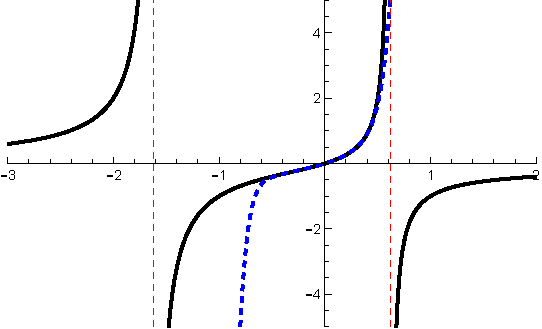
\includegraphics[width=6in]{graph.pdf}
	\end{center}
	Create the figure, formatted exactly as shown. Be efficient when you type the 11\textsuperscript{th} degree polynomial within a \verb|Plot[]| environment.
	\newpage 
	\item With a partner, typeset an exact replica of this document. Your final homework submission must include---all in one file!---the following: 
	\begin{enumerate}
		\item your replica PDF file, generated with \LaTeX
		\item the \textit{Mathematica} file you created 
		\item the \LaTeX \ source code you created.
	\end{enumerate}
\end{enumerate}
\end{document}